\chapter{Introduction}
\label{ch:intro}

\section{Background}
\label{sect:background}

In the early 1990's, there was a lack of quantitative studies for the characterization of a side-dump combustor's flow field. These types of combustors are generally found in solid-propellant ducted rocket ramjets (SDR). In Figure~\ref{fig:config} below, the configuration for such a combustor is shown.

\begin{figure}[H]
	\centering
	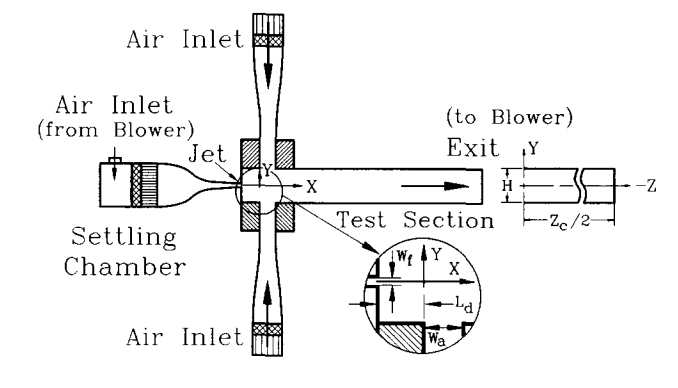
\includegraphics[scale=0.5]{ref/config}
	\caption[Combustor's configuration.]{Combustor's configuration. \cite{art}}
	\label{fig:config}
\end{figure}

Characterization was completed in \cite{art} with laser-Doppler velocimetry (LDV) techniques. Mean velocities, turbulent kinetic energy and Reynolds stresses were measured. This study is used as a precedent for this report.

\section{Purpose}
\label{sect:purpose}

The purpose of this report is  to determine results of side inlet angle variation on the combustor's. mixing abilites \cite{proj}. Specifically counter-clockwise (CCW) and clockwise (CW) angles of -20\textsuperscript{o} and 10\textsuperscript{o} from specified origin, respectively.


\section{Scope}
In this report, the geometry, mesh and set-up for all three models will be presented in the CFX-Pre section. Temperature will be used to determine mixing (passive fluid marker). After this, results for each simulation will be presented. Results will be compared with each other and final conclusions will be made.